\section{Assembly verification: current fitted group9--12}
The present campaign is a functional assembly check. Unmeasured fixtures or missing stimuli do not receive PASS. The current group has two observed discrepancies; this document is not an unconditional board release.

\begingroup\setlength{\tabcolsep}{3pt}\begin{longtable}{>{\raggedright\arraybackslash}p{0.2867\linewidth}>{\raggedright\arraybackslash}p{0.2867\linewidth}>{\raggedright\arraybackslash}p{0.2867\linewidth}}\toprule
Case & Observ\allowbreak{}ed result\allowbreak{} & Dispos\allowbreak{}ition\\\midrule\endhead
CFD monito\allowbreak{}r9/\allowbreak{}10/\allowbreak{}12 & All eight inputs\allowbreak{} pass & PASS\\
CFD monito\allowbreak{}r11 & Raw MUX7=5.479V; other module\allowbreak{}s about3\allowbreak{}.41V & FAIL: fixtur\allowbreak{}e branch\allowbreak{}/\allowbreak{}varian\allowbreak{}t\\
JTAG/\allowbreak{}static\allowbreak{} links & 168/\allowbreak{}168 in each indepe\allowbreak{}ndent path & PASS: scoped\allowbreak{} static\allowbreak{} check\\
CPU/\allowbreak{}FPGA and periph\allowbreak{}erals & 32walk\allowbreak{}ing patter\allowbreak{}ns restor\allowbreak{}ed; IDs/\allowbreak{}PGOOD correc\allowbreak{}t & PASS\\
I2C rails and teleme\allowbreak{}try & Eight popula\allowbreak{}ted rail voltag\allowbreak{}es in nomina\allowbreak{}l window\allowbreak{}s & PASS; nomina\allowbreak{}l curren\allowbreak{}ts\\
Ethern\allowbreak{}et/\allowbreak{}IPbus & 393216\allowbreak{}ADC payloa\allowbreak{}d bytes checke\allowbreak{}d; stable\allowbreak{} ADC/\allowbreak{}TDC transf\allowbreak{}ers & PASS: functi\allowbreak{}onal transp\allowbreak{}ort\\
HDMI data lanes & Walkin\allowbreak{}g,\allowbreak{} slow/\allowbreak{}fast PRBS and idle frames\allowbreak{} correc\allowbreak{}t & Data checks\allowbreak{} PASS\\
HDMI shared\allowbreak{} SPI releas\allowbreak{}e & SYS resets\allowbreak{} after pad releas\allowbreak{}e follow\allowbreak{}ing reads0\allowbreak{}/\allowbreak{}1/\allowbreak{}2 & Overal\allowbreak{}l HDMI FAIL\\
Analog\allowbreak{} channe\allowbreak{}l9 & USB remain\allowbreak{}s on10 & NOT MEASUR\allowbreak{}ED; owner move pendin\allowbreak{}g\\
\bottomrule\end{longtable}\endgroup
\subsection{CFD monitor discrepancy is on the tester}
The emulator at PM position11 (provisional CFD02) gives about5.479V directly at MUX7. Independent revisits reproduce it; position12 gives about3.410V. Check CFD SIM R3=33kOhm to ground, R4=20kOhm from P5V5 and their joints, or confirm an intended assembly variant. The nominal53/33 correction would yield8.80V, but that is not a measured8.80V PM supply. The independent PM INA bus reading is5.496V.

\begin{center}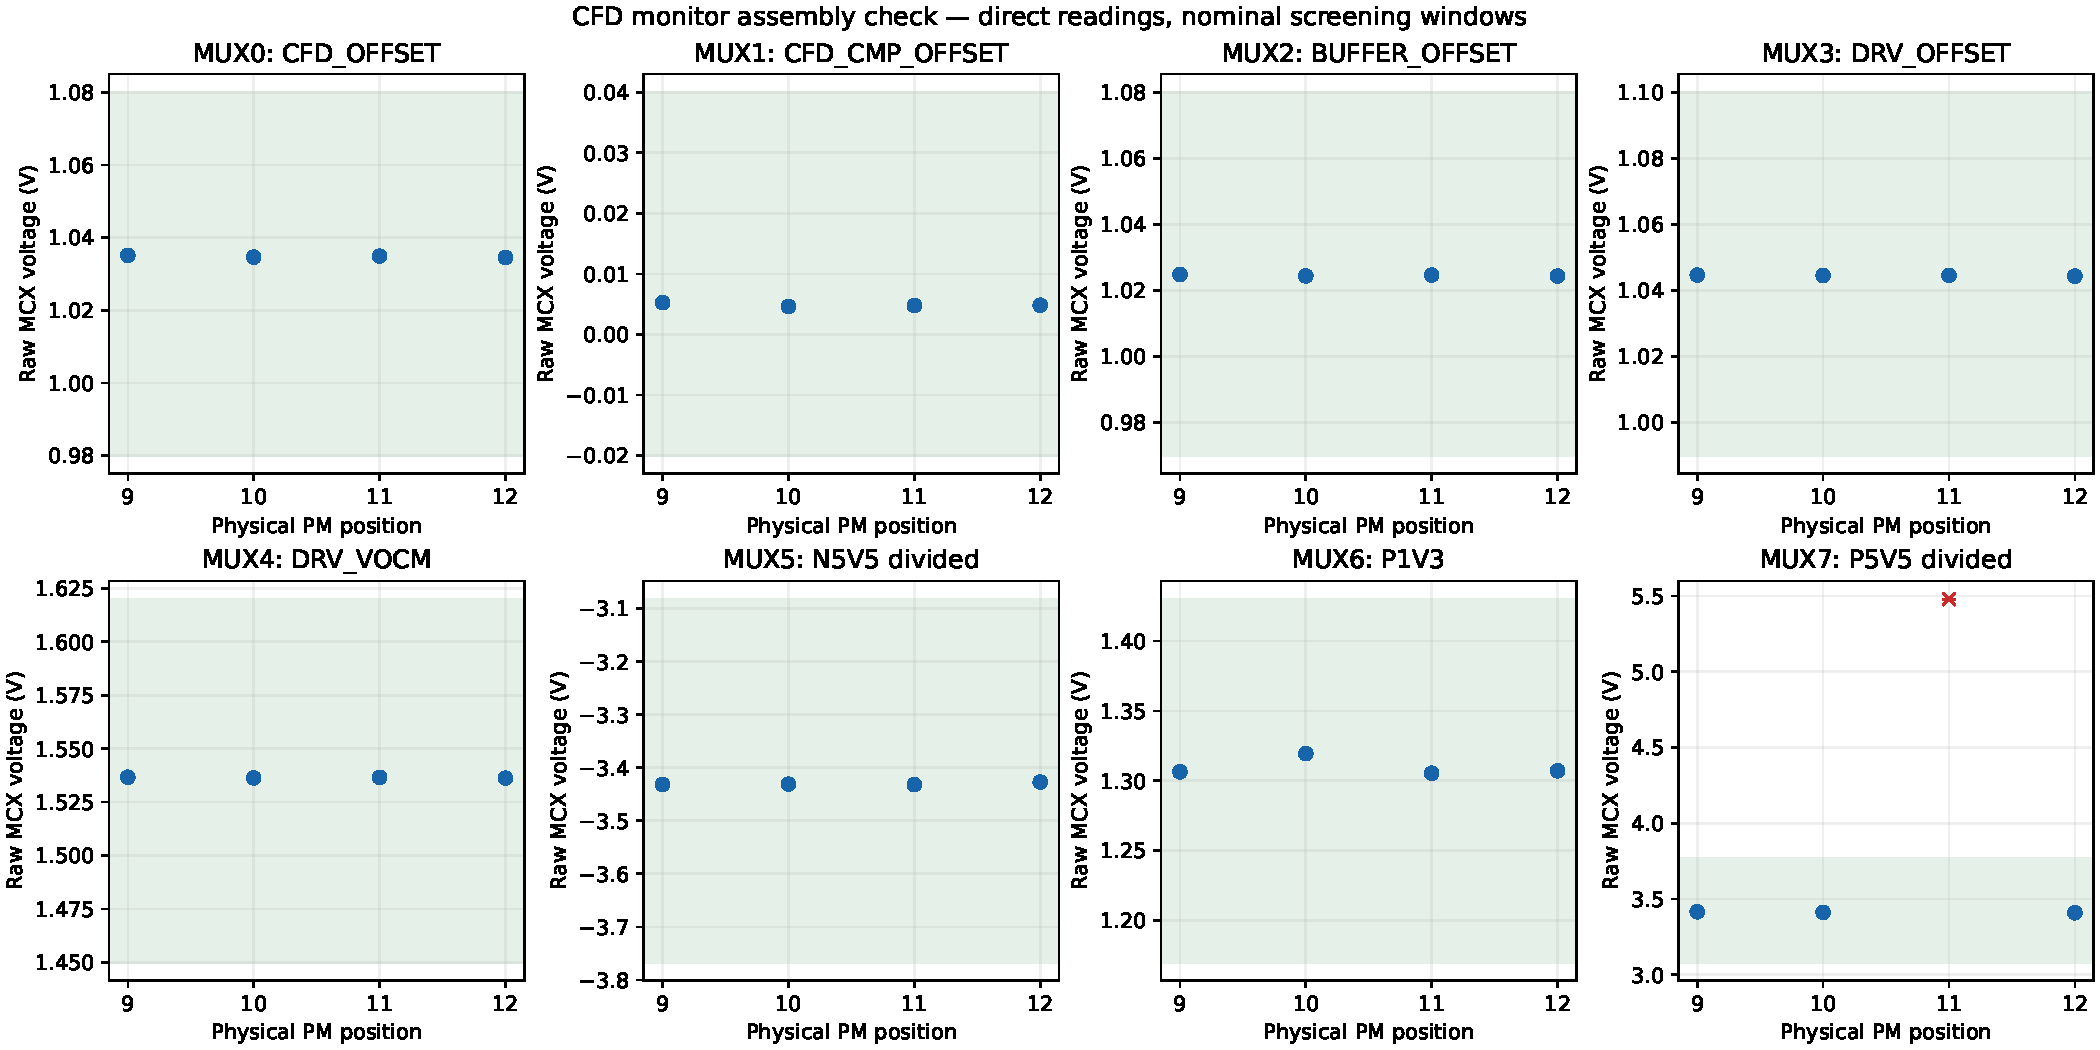
\includegraphics[width=\textwidth]{monitor-assembly.pdf}\end{center}
\begingroup\setlength{\tabcolsep}{3pt}\begin{longtable}{>{\raggedright\arraybackslash}p{0.1433\linewidth}>{\raggedright\arraybackslash}p{0.1433\linewidth}>{\raggedright\arraybackslash}p{0.1433\linewidth}>{\raggedright\arraybackslash}p{0.1433\linewidth}>{\raggedright\arraybackslash}p{0.1433\linewidth}>{\raggedright\arraybackslash}p{0.1433\linewidth}}\toprule
PM positi\allowbreak{}on & Mux & Signal\allowbreak{} & Raw MCX(V) & Nomina\allowbreak{}l equiva\allowbreak{}lent(V) & Screen\allowbreak{}\\\midrule\endhead
9 & 0 & CFD\_\allowbreak{}OFFSET\allowbreak{} & 1.035097\allowbreak{} & 1.035097\allowbreak{} & within\allowbreak{} window\allowbreak{}\\
10 & 0 & CFD\_\allowbreak{}OFFSET\allowbreak{} & 1.034600\allowbreak{} & 1.034600\allowbreak{} & within\allowbreak{} window\allowbreak{}\\
11 & 0 & CFD\_\allowbreak{}OFFSET\allowbreak{} & 1.034880\allowbreak{} & 1.034880\allowbreak{} & within\allowbreak{} window\allowbreak{}\\
12 & 0 & CFD\_\allowbreak{}OFFSET\allowbreak{} & 1.034510\allowbreak{} & 1.034510\allowbreak{} & within\allowbreak{} window\allowbreak{}\\
9 & 1 & CFD\_\allowbreak{}CMP\_\allowbreak{}OFFSET\allowbreak{} & 0.005240\allowbreak{} & 0.005240\allowbreak{} & within\allowbreak{} window\allowbreak{}\\
10 & 1 & CFD\_\allowbreak{}CMP\_\allowbreak{}OFFSET\allowbreak{} & 0.004597\allowbreak{} & 0.004597\allowbreak{} & within\allowbreak{} window\allowbreak{}\\
11 & 1 & CFD\_\allowbreak{}CMP\_\allowbreak{}OFFSET\allowbreak{} & 0.004763\allowbreak{} & 0.004763\allowbreak{} & within\allowbreak{} window\allowbreak{}\\
12 & 1 & CFD\_\allowbreak{}CMP\_\allowbreak{}OFFSET\allowbreak{} & 0.004817\allowbreak{} & 0.004817\allowbreak{} & within\allowbreak{} window\allowbreak{}\\
9 & 2 & BUFFER\allowbreak{}\_\allowbreak{}OFFSET\allowbreak{} & 1.024807\allowbreak{} & 1.024807\allowbreak{} & within\allowbreak{} window\allowbreak{}\\
10 & 2 & BUFFER\allowbreak{}\_\allowbreak{}OFFSET\allowbreak{} & 1.024370\allowbreak{} & 1.024370\allowbreak{} & within\allowbreak{} window\allowbreak{}\\
11 & 2 & BUFFER\allowbreak{}\_\allowbreak{}OFFSET\allowbreak{} & 1.024637\allowbreak{} & 1.024637\allowbreak{} & within\allowbreak{} window\allowbreak{}\\
12 & 2 & BUFFER\allowbreak{}\_\allowbreak{}OFFSET\allowbreak{} & 1.024320\allowbreak{} & 1.024320\allowbreak{} & within\allowbreak{} window\allowbreak{}\\
9 & 3 & DRV\_\allowbreak{}OFFSET\allowbreak{} & 1.044630\allowbreak{} & 1.044630\allowbreak{} & within\allowbreak{} window\allowbreak{}\\
10 & 3 & DRV\_\allowbreak{}OFFSET\allowbreak{} & 1.044490\allowbreak{} & 1.044490\allowbreak{} & within\allowbreak{} window\allowbreak{}\\
11 & 3 & DRV\_\allowbreak{}OFFSET\allowbreak{} & 1.044540\allowbreak{} & 1.044540\allowbreak{} & within\allowbreak{} window\allowbreak{}\\
12 & 3 & DRV\_\allowbreak{}OFFSET\allowbreak{} & 1.044317\allowbreak{} & 1.044317\allowbreak{} & within\allowbreak{} window\allowbreak{}\\
9 & 4 & DRV\_\allowbreak{}VOCM & 1.536640\allowbreak{} & 1.536640\allowbreak{} & within\allowbreak{} window\allowbreak{}\\
10 & 4 & DRV\_\allowbreak{}VOCM & 1.536307\allowbreak{} & 1.536307\allowbreak{} & within\allowbreak{} window\allowbreak{}\\
11 & 4 & DRV\_\allowbreak{}VOCM & 1.536590\allowbreak{} & 1.536590\allowbreak{} & within\allowbreak{} window\allowbreak{}\\
12 & 4 & DRV\_\allowbreak{}VOCM & 1.536213\allowbreak{} & 1.536213\allowbreak{} & within\allowbreak{} window\allowbreak{}\\
9 & 5 & N5V5 divide\allowbreak{}d & -\allowbreak{}3.431790\allowbreak{} & -\allowbreak{}5.511663\allowbreak{} & within\allowbreak{} window\allowbreak{}\\
10 & 5 & N5V5 divide\allowbreak{}d & -\allowbreak{}3.431030\allowbreak{} & -\allowbreak{}5.510442\allowbreak{} & within\allowbreak{} window\allowbreak{}\\
11 & 5 & N5V5 divide\allowbreak{}d & -\allowbreak{}3.431913\allowbreak{} & -\allowbreak{}5.511861\allowbreak{} & within\allowbreak{} window\allowbreak{}\\
12 & 5 & N5V5 divide\allowbreak{}d & -\allowbreak{}3.427043\allowbreak{} & -\allowbreak{}5.504039\allowbreak{} & within\allowbreak{} window\allowbreak{}\\
9 & 6 & P1V3 & 1.306307\allowbreak{} & 1.306307\allowbreak{} & within\allowbreak{} window\allowbreak{}\\
10 & 6 & P1V3 & 1.319360\allowbreak{} & 1.319360\allowbreak{} & within\allowbreak{} window\allowbreak{}\\
11 & 6 & P1V3 & 1.305370\allowbreak{} & 1.305370\allowbreak{} & within\allowbreak{} window\allowbreak{}\\
12 & 6 & P1V3 & 1.307083\allowbreak{} & 1.307083\allowbreak{} & within\allowbreak{} window\allowbreak{}\\
9 & 7 & P5V5 divide\allowbreak{}d & 3.416020\allowbreak{} & 5.486335\allowbreak{} & within\allowbreak{} window\allowbreak{}\\
10 & 7 & P5V5 divide\allowbreak{}d & 3.412337\allowbreak{} & 5.480419\allowbreak{} & within\allowbreak{} window\allowbreak{}\\
11 & 7 & P5V5 divide\allowbreak{}d & 5.479303\allowbreak{} & 8.800093\allowbreak{} & OUTSID\allowbreak{}E WINDOW\allowbreak{}\\
12 & 7 & P5V5 divide\allowbreak{}d & 3.409380\allowbreak{} & 5.475671\allowbreak{} & within\allowbreak{} window\allowbreak{}\\
\bottomrule\end{longtable}\endgroup
Nominal equivalent uses53/33 only for the divided rails. On the failed branch that assumption is suspect; use the direct reading for diagnosis. This is an assembly window check, not traceable calibration or a measurement of analog off-resistance.

\subsection{HDMI reset isolation and restored operating state}
Both full integrated runs retain the unexpected reset. Controlled isolation observes no reset during an idle-only enable/release or during the signature reads themselves. The counter clears when FPGA pads are released after SPI reads, before the DIO direction restoration. The exact electrical/MCU interaction remains unresolved; it must not be called a PM assembly defect solely from this test. Full HDMI remains FAIL until resolved. No arbitrary SPI writes were used.

\begingroup\setlength{\tabcolsep}{3pt}\begin{longtable}{>{\raggedright\arraybackslash}p{0.4300\linewidth}>{\raggedright\arraybackslash}p{0.4300\linewidth}}\toprule
Isolat\allowbreak{}ion event & Raw64-\allowbreak{}bit SYS uptime\allowbreak{}\\\midrule\endhead
initia\allowbreak{}l & 189023\allowbreak{}52588\\
before\allowbreak{} FPGA pad releas\allowbreak{}e & 189023\allowbreak{}57244\\
after FPGA pad releas\allowbreak{}e & 189031\allowbreak{}71692\\
output\allowbreak{}s enable\allowbreak{}d & 189186\allowbreak{}16796\\
idle inside\allowbreak{} & 189186\allowbreak{}21884\\
before\allowbreak{} FPGA pad releas\allowbreak{}e & 189186\allowbreak{}26578\\
after FPGA pad releas\allowbreak{}e & 189194\allowbreak{}43448\\
after idle direct\allowbreak{}ion restor\allowbreak{}e & 189307\allowbreak{}11667\\
before\allowbreak{} FPGA pad releas\allowbreak{}e & 189307\allowbreak{}22089\\
after FPGA pad releas\allowbreak{}e & 189315\allowbreak{}46991\\
output\allowbreak{}s enable\allowbreak{}d & 189470\allowbreak{}31189\\
before\allowbreak{} read 0 & 189470\allowbreak{}35621\\
after read 0 & 189470\allowbreak{}72587\\
before\allowbreak{} read 1 & 189470\allowbreak{}77350\\
after read 1 & 189471\allowbreak{}07457\\
before\allowbreak{} read 2 & 189471\allowbreak{}10108\\
after read 2 & 189471\allowbreak{}37010\\
before\allowbreak{} FPGA pad releas\allowbreak{}e & 189471\allowbreak{}39746\\
after FPGA pad releas\allowbreak{}e & 405695\allowbreak{}38\\
after SPI direct\allowbreak{}ion restor\allowbreak{}e & 518880\allowbreak{}40\\
before\allowbreak{} FPGA pad releas\allowbreak{}e & 518943\allowbreak{}23\\
after FPGA pad releas\allowbreak{}e & 527136\allowbreak{}83\\
\bottomrule\end{longtable}\endgroup
After isolation, fresh ADC and TDC transport checks passed with no SYS reset. The JTAG wrapper retains its ERROR from the combined HDMI guard; JTAG PASS here comes from independently rebuilt static vectors and checksum-verified restored SRAM followed by those stable checks. The separate HDMI failure remains visible.

Firmware still prints the old R15-not-fitted label for P3V8. The owner confirmed R15 fitted; the schematic specifies1mOhm. Host conversion of the retained signed shunt code at40uV/LSB gives about3.12A, uncalibrated. The original firmware text is retained. No MCU firmware was changed; route6/channel3 is unpopulated and excluded. Power-sequence fault injection is not performed.

Final state: qualified c7c42d28 diagnostic in FPGA SRAM, private PM bridge active, HDMI/CFD outputs released, DIO cards input, ADC bankA physical capture and frozen quiet TDC. SMU OFF/HIZ at0A, all four monitor muxes inhibited and TCA masks0. USB cables stay on10. Prior analog measurements retain their own acquisition settings; they are not silently remeasured after reconfiguration.
